\documentclass{article}

\usepackage[utf8]{inputenc}
\usepackage{ngerman}
\usepackage{lmodern}
\usepackage{amsthm}
\usepackage{amssymb}
\usepackage{amsmath}
\usepackage[paper=a4paper,left=25mm,right=25mm,top=25mm]{geometry}
\usepackage{mathtools}
\usepackage{graphicx}

\newtheorem{satz}{Satz}
\newtheorem{definition}[satz]{Definition}
\newtheorem{lemma}[satz]{Lemma}
\newtheorem{proposition}[satz]{Proposition}
%Create a new theorem by writing \newtheorem{How to call this type of theorem}[satz]{What should be written}. Make sure to keep "satz" to ensure consecutive numeration.
% %  Variablen Definition...............
\newcommand*{\R}{k[X_{1},\ldots,X_{n}]}
\newcommand*{\I}{I_{\leq s}}
\newcommand*{\indx}[2]{{#1}_{#2}}
\newcommand*{\potx}[2]{{#1}^{#2}}
\newcommand*{\N}{\mathrm{N}_0}
\newcommand*{\hf}[1]{$\prescript{a}{}{HF}_{#1}$}
\newcommand*{\hp}[1]{$\prescript{a}{}{HP}_{#1}$}
\newcommand*{\kette}[2]{$1\leq {#1}_1<{#1}_2<{#1}_3<...<{#1}_{#2}\leq n$}
\newcommand*{\Rr}[2]{$ k[X_{{#1}_{1}},\ldots,X_{{#1}_{#2}}]$}
%\newcommand*{\hf}{}
\newcommand*{\ideal}{$I$}


\title{Dimension von Varietäten}
\date{\today}
\author{Yvan Ngumeteh \and Emma Ahrens}

\begin{document}

\maketitle
\tableofcontents

\section{Abstract}
\section{Einleitung}
\section{Dimension von Monomidealen}

	\begin{lemma} \label{1.2.3}
	Sei \(I \subseteq \R\) ein Ideal, das von einer Menge G von Monomen erzeugt wird. Dann liegt
	ein Polynom \(f \in \R\) in I genau dann, wenn für jeden Term \(a_{j}X^{\alpha_{j}}\) von f ein
	\(g \in G\) existiert, welches \(a_{j}X^{\alpha_{j}}\) teilt.
	\end{lemma}

	\begin{proof}[Beweis]
	Sei \(f \in I\). Dann gilt \(f = \sum_{i=1}^{s} h_{i}g_{i}\) mit \(h_{i} \in R\) und \(g_{i}
	\in G\). Damit hat jeder Term die Form \(h_{i}g_{i}\) und ist somit durch ein Element aus G
	teilbar.
	Sei nun andersherum \(f \in \R\) und für jeden Term \(a_{j}X^{\alpha_{j}}\) von f existiert ein
	\(g \in G\), welches \(a_{j}X^{\alpha_{j}}\) teilt. Dann kann man f als Linearkombination von 
	Elementen aus G schreiben und damit liegt f nach der Definition eines Ideals in I.
	\end{proof}

	
	\begin{lemma} \label{1.2.4}
	Sei \((g_{i})_{i \geq 1}\) eine Folge von Monomen in \(\R\) mit \(g_{1} \succeq g_{2} \succeq
	\ldots\) für eine Monomialordnung \(\preceq\). Dann existiert ein \(r \in \mathbb{N}\) mit 
	\(g_{n} = g_{r}\) für alle \(n \geq r\). 
	\end{lemma}

	\begin{proof}[Beweis]
	Sei \(I = ((g_{i})_{i \geq 1})\), dann ist I ein Ideal. Nach dem Hilbert'schen Basissatz
	wissen wir, dass I endlich erzeugt ist. Also existiert ein r, so dass die Menge \(G = \{g_{1},
	\ldots, g_{r}\}\) I erzeugt. Für ein \(i \geq r\) und \(g_{i} \in I\) existiert ein
	\(j \in \underline{r}\), so dass \(g_{j}\; | \;(g_{i}\) nach Lemma~\ref{1.2.3}. Also \(g_{i}
	\succeq g_{j} \succeq g_{r}\). Andererseits gilt nach Voraussetzung, dass \(g_{i} \preceq g_{r}
	\), also folgt \(g_{i} = g_{r}\).
	\end{proof}

	Lemma~\ref{1.2.4} sagt uns, dass jede absteigende Kette von Monomen stationär wird und
	insbesondere in jeder abzählbaren Menge von Monomen ein kleinstes Element existiert.
	

	\begin{proposition}[Divisionsalgorithmus] \label{1.2.5}
	Sei \(\preceq\) eine Monomialordnung und \(f, f_{1}, \ldots, f_{s} \in \R\) nicht null. Dann
	gilt \begin{displaymath} f = \sum_{i=1}^{s} h_{i}f_{i}\; + r, \end{displaymath} mit
	\(r, h_{1}, \ldots, h_{s} \in \R\) und \(LT(h_{i}f_{i} \preceq LT(f)\) für alle \(h_{i} \neq 0
	\) und \(r = 0\) oder kein Term von r wird durch ein \(LT(f_{i})\) geteilt für \(i \in
	\underline{s}\).
	\end{proposition}

	\begin{proof}[Beweis]
	Wir beweisen diese Proposition per TODO downward Induktion über LT(f). \\
	Beim Induktionsschritt unterscheiden wir drei Fälle:\\
	Sei f konstant, dann gilt \(f = \sum_{i=1}^{s} 0f_{i}\; + r\) mit \(r := f\) und \(h_{i} := 0\). \\
	Falls ein \(i \in \underline{s}\) existiert, so dass \(LT(f_{i})\;| \; LT(f)\), setzen wir
	\begin{displaymath} f^{(1)} := f - \frac{LT(f)}{LT(f_{i})}f_{i}.\end{displaymath} Dann gilt
	\( f = f^{(1)} + \frac{LT(f)}{LT(f_{i})}f_{i} \) mit \(h_{i} = \frac{LT(f)}{LT(f_{i})}\) und 
	\(LT(h_{i}f_{i}) = LT(f) \preceq LT(f).\) \\
	Falls kein solches \(f_{i}\) existiert, schreiben wir \begin{displaymath} f^{(1)} := f -
	LT(f). \end{displaymath} Und \(f = f^{(1)} + LT(f)\) mit \(r = LT(f)\) erfüllt die Bedingungen 
	(insbesondere, dass kein Term von r durch ein \(LT(f_{i})\) geteilt wird). \\
	Führe den Schritt nun induktiv auf \(f^{(1)}\) durch bis \(f^{(j)} = 0\) und bestimme
	\(h_{1}, \ldots, h_{s}, r\) durch Rückwärtseinsetzen.
	\end{proof}

	
	Evtl. Beispiel, dass diese Form nicht eindeutig ist.


	\begin{satz} \label{1.2.8}
	Sei \(\{0\} \neq I \subseteq \R\) ein Ideal und \(\preceq\) eine Monomialordnung auf
	\(Z^{n}_{\geq 0}\). Sei G eine Gröbnerbasis von I mit I = (G). Dann ist eine k-Basis von 
	\(\R/I\) gegeben durch die Restklassen von \(X^{\alpha}\) mit
	\begin{displaymath}
	\alpha \in C(I) := \{\alpha \in Z^{n}_{\geq 0}\, |\; LT(g) \nmid X^{\alpha}\quad \forall g 
	\in G\}.
	\end{displaymath}
	\end{satz}

	\begin{proof}[Beweis]
	Wir zeigen erst, dass die Monome mit Exponent aus C(I) ganz \(k[X_{1},\ldots,X_{n}]/I\) 
	aufspannen und anschließend, dass kein Element aus I durch echte Linearkombination solcher
	Monome dargestellt werden kann. \\
	Sei \(G = \{f_{1}, \ldots, f_{s}\}\) und \(0 \neq f \in \R\). Dann ist
	\(f = \sum_{i=1}^{s} h_{i}f_{i}\; + r = f' + r\) nach Proposition~\ref{1.2.5} mit \(r=0\) oder 
	\(r = a_{l}X^{\alpha_{l}} + \ldots + a_{0}\) mit \(LT(f_{i}) \nmid X^{\alpha_{j}}\) 
	für jedes \(i \in \underline{s}\) und \(j \in \underline{l}\). Also ist \(r\) eine
	Linearkombination von Monomen \(X^{\alpha_{j}}\) mit \(\alpha_{j} \in C(I)\).
	Es gilt außerdem \([f] = [r]\) in \(\R/(G)\) und damit erzeugen die
	Monome mit \(\alpha \in C(I)\) den ganzen Restklassenring. \\
	Angenommen es existiert \(f = f' + r \in I\) mit \(r \neq 0\) und f' und r wie oben.
	Dann gilt \(0 \neq r = f - f'\). Da \(f \in I\) und \(f' \in I\) folgt
	\(r \in I\), womit folgt, dass \((LT(r) \in (LT(f_{1}), \ldots, LT(f_{s}))\).
	Nach Lemma~\ref{1.2.3} existiert dann ein \(f_{i}\) mit \(LT(f_{i})\; |\; LT(r)\). Dies ist 
	ein Widerspruch, also folgt \(r = 0\) und die Restklassen von \(X^{\alpha}\) mit
	\(\alpha \in C(I)\) sind linear unabhängig in \(\R/I\).
	\end{proof}
	
	Was sagt uns Beispiel 1.2.9?? TODO

	\begin{center}
	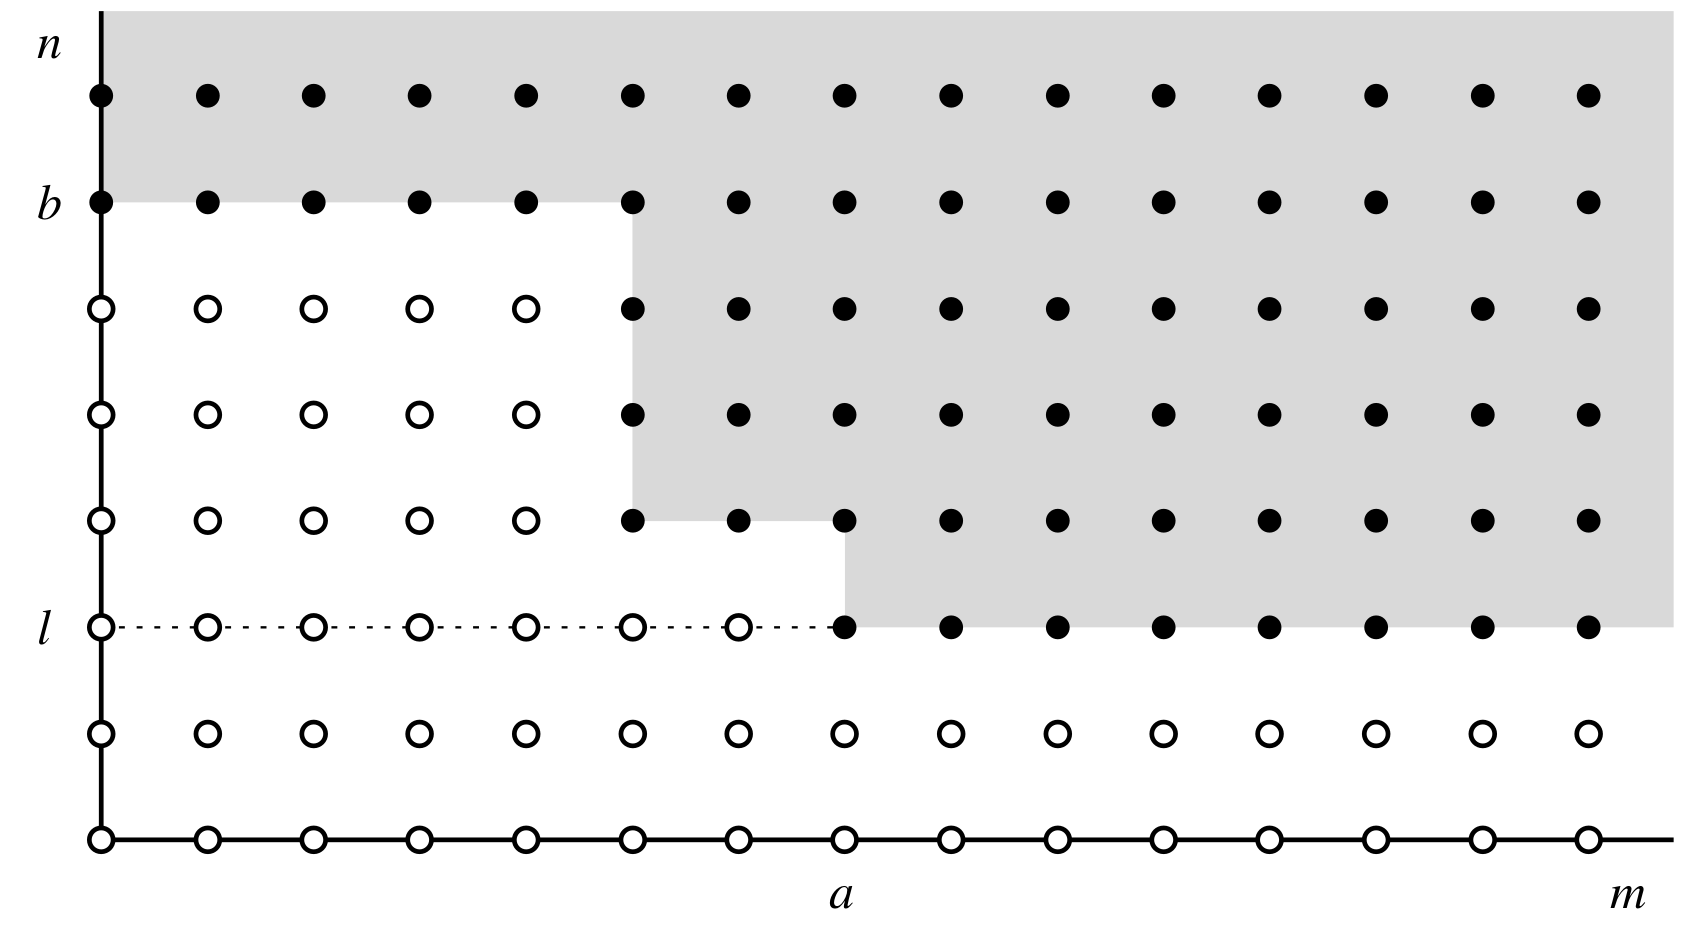
\includegraphics[width=.75\linewidth]{Dots.png}
	\end{center}

	\begin{figure}[h]
		\centering
		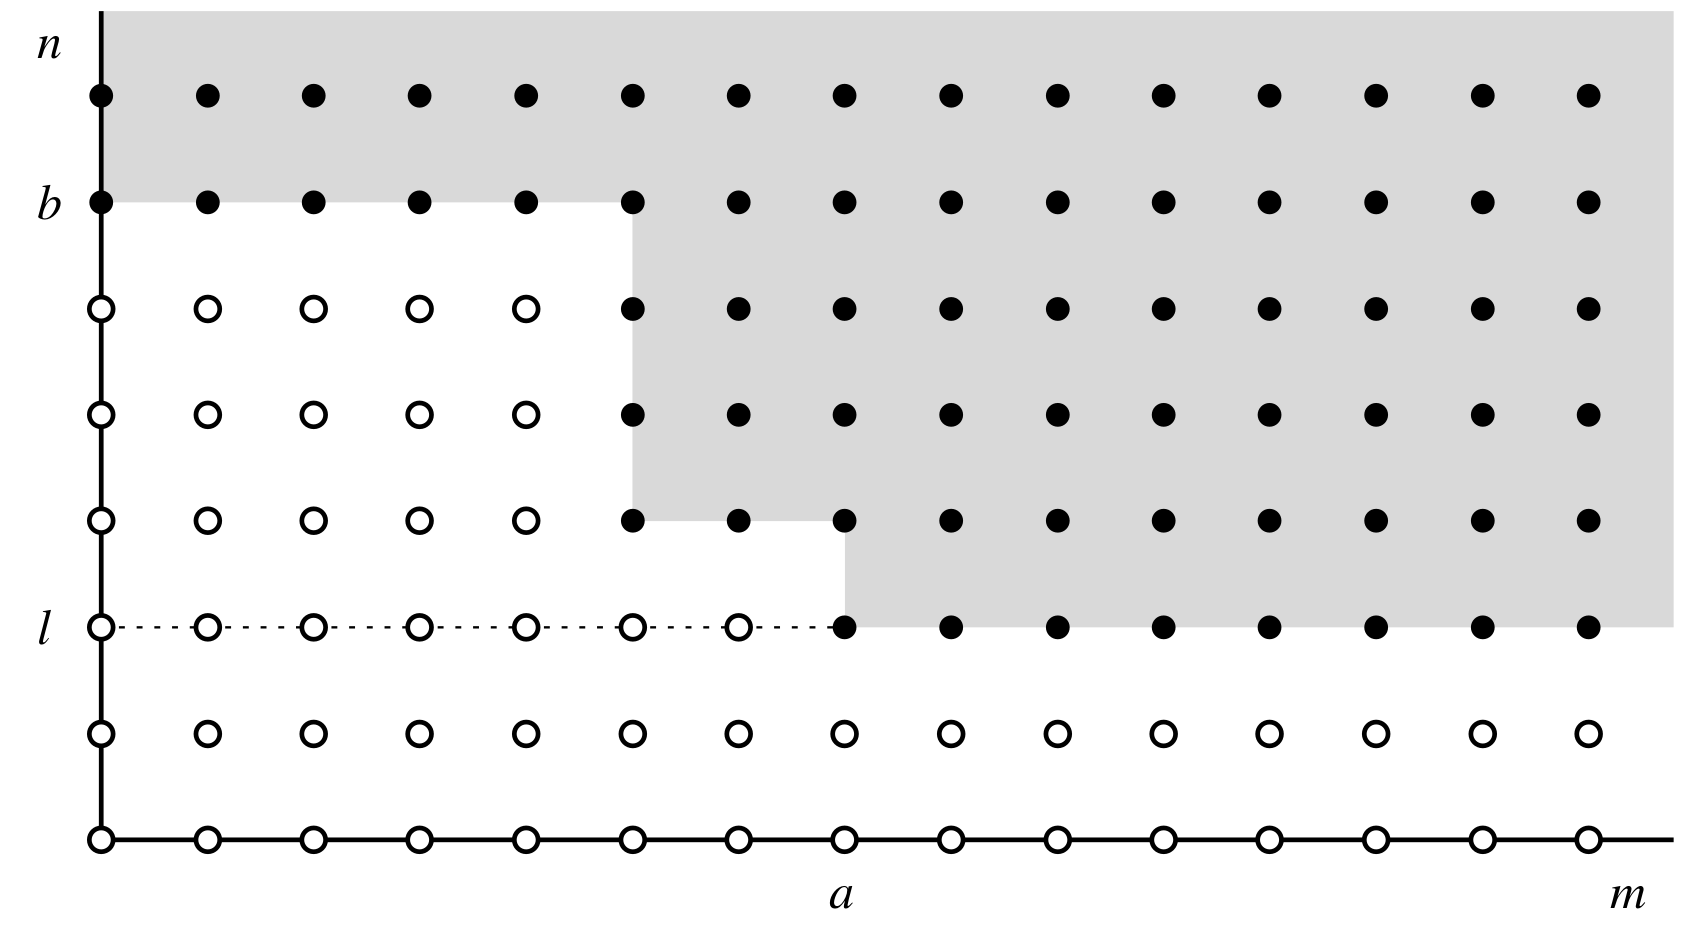
\includegraphics[width=.75\linewidth]{Dots.png}
		\caption{Anschauliche Darstellung von \(\R/I\) aus \cite{CLOS}}
		\label{dots}
	\end{figure}
	
	Bildchen mit Punkten und Erklärung dazu.
	Wir betrachten das \''Wachstum\'' von \(\R/I\)

	\begin{definition} \label{1.2.11}
	Sei \(I \subseteq \R\) ein Ideal und \(s \in \mathbb{N}_{0}\). Dann definiere \(I_{\leq s} :=
	I \cap \R_{\leq s}\). Nun gilt, dass \(\R_{\leq s}\) ein endlich dimensionaler Vektorraum über
	k  mit \(I_{\leq s}\) als Teilraum ist. Wir können die Funktion \begin{displaymath}
	\prescript{a}{}{HF}_{I} : \mathbb{N}_{0} \rightarrow \mathbb{N}_{0}, \quad s \mapsto
	dim_{k}(\R_{\leq s}/I_{\leq s})	\end{displaymath} definieren, die (affine) Hilbertfunktion
	von I genannt wird.
	\end{definition}


	\paragraph{Ein paar Beispiele}
	\begin{itemize}
	\item Sei \(I = \R\). Dann ist
		\begin{align*}
			\prescript{a}{}{HF}_{I}(s) &= dim_{k}(\R_{\leq s}/I_{\leq s}) \\
			&= dim_{k}(\R_{\leq s}/\R_{\leq s}) \\
			&= dim_{k}(\emptyset) \\
			&= 0
		\end{align*}
	 für alle \(s \in \mathbb{N}_{0}\).  
	\item Sei nun \(I = \{0\}\). Dann ist
		\begin{align*}
			\prescript{a}{}{HF}_{I}(s) &= dim_{k}(\R_{\leq s}/I_{\leq s}) \\
			&= dim_{k}(\R_{\leq s}) \\
			&= |\{ X^{\alpha} \in Z^{n}_{\geq 0}\, |\; |\alpha| \leq s\}| \\
			&= \sum_{i=1}^{s} |\{ X^{\alpha} \in Z^{n}_{\geq 0}\, |\; |\alpha| = i\}| \\
			&= TODO \\
			&= \sum_{i=1}^{s} \binom{n-1+k}{k} \\
			&= \binom{s+n}{s} = \binom{s+n}{n} \\
			&= \frac{1}{n!}(s+n)(s+n-1)\cdots (s+1) \\
			&= \frac{1}{n!}s^{n} + \frac{1}{n!}\binom{n+1}{2}s^{n-1} + \cdots + 1. \\
		\end{align*}
	Zu beachten ist hier, dass der Grad der Hilbertfunktion n ist, also der Dimension von \(\R/I\)
	entspricht. Dies werden wir im Folgenden näher betrachten.
	\item Einfaches Beispiel aus CLOS. TODO
	\end{itemize}
	

	\begin{lemma}[Macaulay] \label{1.2.13}
	Sei \(\preceq\) eine gradierte lexikographische Monomialordnung und \(I \subseteq \R\) ein
	Ideal. Dann ist \(\prescript{a}{}{HF}_{I}(s) = \prescript{a}{}{HF}_{LT(I)}(s)\) für alle
	\(s \in \mathbb{N}_{0}\).
	\end{lemma}

	
	\begin{proof}[Beweis]
	Zunächst definieren wir uns die Menge
	\begin{displaymath}
		D := \{LM(f)\; |\; 0 \neq f \in \I\} = \{LM(f_{1}), \ldots, LM(f_{m})\}
	\end{displaymath}
	für ein \(m \in \mathbb{N}_{0}\) und \(f_{i} \in \I\) für alle \(i \in \underline{m}\). Die
	zweite Gleichheit gilt aufgrund der Endlichkeit von \(\I\).
	Wir betrachten außerdem die Menge
	\begin{displaymath} B := \{f_{1}, \ldots, f_{m}\}. \end{displaymath}
	Die Elemente aus B entsprechen denen aus der Menge D.

	Wir zeigen nun, dass D eine k-Basis von \((LT(I))_{\leq s}\) und B eine k-Basis von \(\I\) ist.
	Dann folgt nämlich, dass die beiden Mengen die selbe Kardinalität und die erzeugten
	Vektorräume die selbe Dimension haben, womit das Lemma von Macaulay gezeigt ist.

	Als Erstes wollen wir zeigen, dass D eine k-Basis von \((LT(I))_{\leq s}\) ist. Da D die
	Leitmonome der Elemente aus I enthält, ist D offensichtlich linear unabhängig.
	Wir zeigen also, dass das Erzeugnis von D ganz \((LT(I))_{\leq s}\) aufspannt: Dazu
	betrachten wir ein beliebiges \(g \in (LT(I))_{\leq s}\). Es gilt \(deg(g) \leq s\) und da D
	alle \(LT(I)\) mit Grad \(\leq s\) enthält, kann man schreiben 
	\(g = \sum_{i=1}^{m} h_{i}LT(f_{i})\) mit \(h_{i} \in k\) für alle \(i \in \underline{m}\).
	Also ist \(g \in (D)\) und damit spannt D ganz \((LT(I))_{\leq s}\) auf. Es folgt also, dass
	D eine k-Basis von \((LT(I))_{\leq s}\) ist.
	
	Jetzt zeigen wir, dass B eine k-Basis von \(\I\) ist. Die lineare Unabhängigkeit der einzelnen 
	Elemente können wir durch einen einfachen Widerspruchsbeweis zeigen:
	Sei \(0 = \sum_{i=1}^{m} h_{i}f_{i}\), \(h_{i} \in k\) für alle \(i \in \underline{m}\),
	und es existiert ein \(i \in \underline{m}\) mit \(h_{i} \neq 0\).
	Da \(f_{i} \neq 0\) ist, existiert mindestens ein \(i \neq j \in \underline
	{m}\) mit \(h_{j} \neq 0\). Ohne Beschränkung der Allgemeinheit kann man annehmen, dass genau
	zwei Koeffizienten \(\neq 0\) existieren. Dann gilt
	\begin{align*}
		0 &= \sum_{i=1}^{m} h_{i}f_{i} = h_{i}f_{i} + h_{j}f_{j} \\
		&\Leftrightarrow -h_{j}f_{j} = h_{i}f_{i} \\
		&\Leftrightarrow -\frac{h_{j}}{h_{i}} f_{j} = f_{i}.
	\end{align*}
	Also gilt \(LM(f_{j}) = LM(f_{i})\), dies ist aber ein Widerspruch zur Definition der Menge B,
	also ist B linear unabhängig. \\
	Wir wählen nun ein \(g \in \I\). Dann existiert ein \(i \in \underline{m}\) mit \(LM(f) =
	LM(f_{i})\), weil \(f \in \I\), also auch \(LM(f) \in D\). Wir definieren
	\begin{align*}
		f^{(1)} := f - \frac{LM(f)}{LM(f_{i})}f_{i} \\
		\Leftrightarrow f = f^{(1)} + \frac{LM(f)}{LM(f_{i})}f_{i}.
	\end{align*}
	Es gilt \(LM(f) = LM(\frac{LM(f)}{LM(f_{i})}f_{i})\), also folgt \(LM(f^{(1)}) \preceq LM(f)\),
	da wir die Monome unter gradierter lexikographischer Ordnung betrachten.
	Für \(f^{(1)}\) existiert wie für f wieder ein \(j \in \underline{m}\) mit \(LM(f) =
	LM(f_{j})\), da \(f^{(1)} \in \I\). Wir definieren \(f^{(2)}\) analog zu oben und es
	folgt \(LM(f^{(2)}) \preceq LM(f^{(1)})\). Das machen wir induktiv weiter bis \(f^{(l)} = 0\)  
	für ein \(l \in \mathbb{N}\).
	Der Algorithmus endet nach endlich vielen Iterationen, da \(LM(f) \succeq LM(f^{(1)}) \succeq LM(f^{(2)}) \succeq \cdots\).
	Also kann man g als k-Linearkombination von Elementen aus B schreiben, damit spannt B ganz \(\I\) und B ist eine Basis von \(\I\).
	\end{proof}


\section{Dimension von beliebigen Idealen}

\subsection{Das Hilbert-Polynom}

Im folgenden sei $n \in \mathrm{N}$ fest.

\begin{satz}
	Sei  \ideal $\subset$ $\R$, dann existiert es einen eindeutigen Polynom \hp{I}(t) $\in \mathrm{Q}[t]$ (mit t eine variable) und $\indx{s}{0}\geq0$,  sodass \hp{I}(s)=\hf{I}(s)= $\indx{dim}{k}$ ($\indx{\R}{\leq s}$/$\indx{I}{\leq s}$), $\forall s\geq\indx{s}{0}$. Weiterhin besitzt \hp{I}(t) folgende Eigenschaften:	
\end{satz}
\begin{itemize}
	\item Der Grad von \hp{I}(t) ist der größte $d \in \mathrm{N}$, sodass es \kette{i}{d} existieren mit $I\cap k[X_{{i}_{1}},\ldots,X_{{i}_{d}}]={\emptyset}$.
	\item Sei $d=grad(\textnormal{\hp{I}(t)})$. Dann gilt \hp{I}(t)=$\sum_{k=0}^{d} \indx{a}{k}t^k$ mit $\indx{a}{k}d! \in \mathrm{Z}, \forall k\in \underline{\indx{d}{0}}$ und $\indx{a}{k}d!>0$
\end{itemize}

\begin{proof}[Beweis]
	Wir bemerken dass \hp{I}(t) eindeutig ist, da es ein Polynom ist. Es nur die Existenz nachgewiesen werden. Sei $M=\{\alpha \in \N:|\alpha|\leq s\}$
	\begin{itemize}
		\item Für die trivialen Fällen $I=(0)$ hat man, wegen \hf{I}(s)= $\indx{dim}{k}$ ($\indx{\R}{\leq s}$/$\indx{I}{\leq s}$)$=$ $\left|M\right|=\binom{n+s}{s}, \forall s\in \N$.
		
		Oder $I=\R$ gilt \hf{I}(s)= $\indx{dim}{k}$ ($\indx{\R}{\leq s}$/$\indx{I}{\leq s}$)$=0, \forall s\in \N$ und somit entspricht in diesem Fall \hp{I}$=0$ (Das Nullpolynom !)
		Nehmen wir also an, dass $I$ nicht trivial ist. Sei G eine Gröbner-Basis von $I$ (bzgl. eine graduierte lexikographische Ordnung) und 
		\begin{displaymath}
		\{LM(g):g\in G\}=\{\indx{X}{\beta}:\beta \in M \}
		\end{displaymath}
		
		wir setzen
		\begin{displaymath}
		C(I):=\{\alpha \in \N: \potx{X}{\beta} \nmid \potx{X}{\alpha} \forall \in \beta \in M \}
		\textnormal{ und } 
		\indx{C(I)}{\leq s}:= C(I) \cap \{\alpha \in \N:|\alpha|\leq s\}
		\end{displaymath}
		
Behauptung: Für $s\geq 0$ gilt \hf{I}(s)$=|\indx{C(I)}{\leq s}|$, $\forall s\geq 0$.

Für den Beweis benutzt man (Macaulay), dann gilt \hf{I}(s)=\hf{(LT(I))}(s), $\forall \in s\geq0$. Das heißt,
\begin{displaymath}
\indx{dim}{k} (\indx{\R}{\leq s}/\indx{I}{\leq s})=\indx{dim}{k}(\indx{\R}{\leq s}/\indx{(LT(I))}{\leq s}).
\end{displaymath}

Weiterhin gilt mit der Buchberger-Definition (1.2.7), dass $\{\potx{X}{\beta}:\beta \in M \}$ ist eine Gröebner-Basis von (LT(I)), deshalb mit Satz 1.2.8 habt man, dass die Restklassen von $\potx{X}{\beta}$ ($\alpha\in C(I)$) bilden eine K-Vektorraum Basis von $\R$/(LT(I)). Daraus folgt die Behauptung.

\item Sei $J\subseteq \underline{n}$ und eine Funktion $\tau:J\longrightarrow \N$. Wir definieren
\begin{displaymath}
C(J,\tau):=\{\alpha \in N: \indx{\alpha}{j}=\tau(j), \forall \in J  \}
\end{displaymath}

Behauptung: Es existiert eine endliche Anzahl $\chi$ von Tupeln (J,$\tau$), sodass 

\begin{displaymath}
C(I)=\bigcup\limits_{(J,\tau)\in \chi}
\end{displaymath}

\begin{proof}
	Für $\beta:=(\indx{\beta}{1},\ldots,\indx{\beta}{n}) \in \N$, definiert man 
	
	\begin{displaymath}
	C(\beta):=\{\alpha\in \potx{\N}{n}: \potx{X}{\beta}\nmid\potx{X}{\alpha}\}
	\end{displaymath}
	Dann haben wir $C(I)=\bigcap\limits_{\beta\in M}C(\beta)$. 
	Weiterhin bemerken wir, dass falls $(J,\tau),(J\prime,\tau\prime)$ zwei Tupeln, wie oben definiert bezeichnet, dann gilt 
	
	\begin{displaymath}
	C(J,\tau)\cap C(J\prime,\tau\prime)=\left\{\begin{array}{ll} \emptyset, & falls  \tau(j)=\tau\prime(j) \\
	C(J\cup J\prime, \tau_0), & sonst \end{array}\right.
	\end{displaymath} 
	wobei $\indx{\tau}{0}:J\cup J\prime \longrightarrow \N$, $ j\mapsto \tau_{0}(j)=\left\{\begin{array}{ll} \tau(j), & falls  j\in J \\
	\tau\prime(j), & falls  j\in J\prime \\
	0, & sonst \end{array}\right.$.
	
	Das heißt man kann O.B.d.A annehmen, dass in 
 	
\end{proof}[Beweis]
	\end{itemize}
\end{proof}
%\minisec{Behauptung}	




\begin{thebibliography}{99}
	\bibitem{Heu03}
	\textsc{Heuser}, Harro:
	\newblock \emph{Lehrbuch der Analysis}.
	\newblock 15. Aufl.
	\newblock Vieweg-Verlag, Braunschweig-Wiesbaden, 2003
	
	\bibitem{GM-GM}
	\textsc{Gr{\"o}ger}, Detlef ; \textsc{Marti}, Kurt:
	\newblock \emph{Grundkurs Mathematik für Ingenieure, Natur- und
		Wirtschaftswissenschaftler}.
	\newblock 2.~Aufl.
	\newblock Physica-Verlag, 2004

	\bibitem{CLOS}
	\textsc{Cox}, David; \textsc{Little}, John; \textsc{O'Shea}, Donal:
	\newblock \emph{Ideals, Varieties, and Algorithms}.
	\newblock Third Edition
	\newblock Springer-Verlag, 2007
\end{thebibliography}


\end{document}
